%This is the last chapter 
%%=========================================
\chapter{Summary}
Overall most of the Re* research components have similar ideas, approaches, and standard practices. In this part, all characteristics will be generalized, made clear differences and general recommendations which should satisfy all of the criteria.\par
First of all, a broad picture of all Re* research characteristics together was made. The central definition is \textbf{recomputability} which refers to the code reusability. Recomputability require having the code and underlying documentation available online that everyone can have access and reuse computation approaches with any data. \textbf{Reproducibility} is inheriting the recomputability characteristic. The basic definition refers to the ability to have similar results with the same code and data sets so that the paper reviewer or researchers from other groups will be able to confirm results. The last characteristic which is aimed to give similar data results(data sets) is \textbf{repeatability}. It is required to have the full description of experimental setup that everyone can get the same results. Of course, it is not possible in real life to get the same results from repeating an experiment, and usually, this characteristic refers to the authors themselves so the experiment will be repeatedly done with the same setup and have in the end deviations adequately done.  Another feature which inhering recomputability is \textbf{replicability}. The main idea of replicability has the same methods which were used to get the result data and codebase documented that no matter what kind of data was used by the initial author other research groups will reach similar conclusions of the particular problem. More complex characteristic is \textbf{reusability} which is by the end of the day means that all data can be reused by anyone else hand having thoroughly everything documented starting from the codebase and initial data and finishing with methods, benchmarks, and approaches. The main idea of reusability can reuse all of this components and make completely new ideas\ref{fig:relationdiagram}.\par
\begin{figure}[h!]
  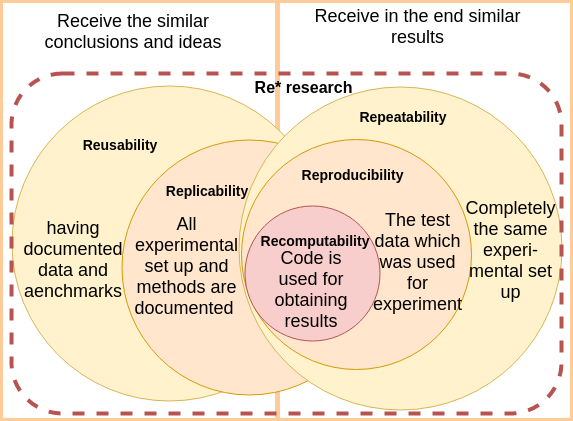
\includegraphics[scale=0.7]{fig/relationdiagram.png}
  \caption{Relation diagram\cite{gith}}
  \label{fig:relationdiagram}
\end{figure}
As can be seen, two characteristics for which includes all other aims, concepts and satisfied criteria are Repeatability and Reusability.
\section{Good practices}
\begin{itemize}
    \item \textbf{Codebase.} computation-based experiments have the critical issue of having everything published and use as long as it possible only open source components. Everything should be documented and work out of the box. Using Docker image would be the good solution for this. Always leave links in the paper where the sources can be found.
    \item \textbf{Experimental set-up.} All hardware and software characteristics should be well described in the paper. For having similar software setup sharing the virtual machine image would solve most of the problems. It is more difficult for having the same hardware setup. To solve this problem all experiments can be done in a virtual machine, and the virtual machine image can be shared afterward. 
    \item \textbf{Experiments.}  Both datasets initial the same as result ones should be in open access. Also, all benchmarks and methods should be documented. 
    \item \textbf{Documentation.} Complete workflow, processes, and problems should be fully documented and provided together with the paper.
\end{itemize}
\section{Important workflows}
\begin{itemize}
    \item \textbf{Statistical methods.} Observable phenomena postulate hypotheses about and then measure. In system studies, the usual performance is the performance measured by the execution time. Some factors include many factors based on the architecture, operating system, compiler, and application. Some elements are controlled by the experimenter (i.e., architecture, compiler parameters or the time of the experiment). There are uncontrollable factors, some of which can be observed, and some of them can not. All independent elements should be randomized. Some parts of the experiment may be beyond the control of the experimenter. Real-time systems respond to real-world incentives, which are themselves random.
    \item \textbf{Documentation.} Proper archiving and documentation allow this even after a long time after the actual hardware or software infrastructure for repeating the experiment becomes unavailable. Indeed, this can also lead to negative results, such as the detection of errors in earlier experiments. The community must provide means of correcting published documents for these cases.
    \item \textbf{Benchmarks.} Experimental studies in systems are based on control applications. The test is a factor in the experiment, like everything else. When the experiment is started only in one of the stages, the value of interest is measured just for this test. If the standard is an application that the user wants to run, then this is normal (modulo). Otherwise, to make more general conclusions, the control factor should also be randomized: work with a variety of different criteria that are representative of real applications and statistically summarize the results.
\end{itemize}
\section{Software solutions}
There are plenty of solutions made to solve Re* research problem not only in computation-based works, this software solutions are evaluated and compared on table\ref{table:comp_table}:
\begin{itemize}
    \item \textbf{PopperCI}\cite{DBLP:conf/infocom/JimenezAALMMR17}: Continuous Integration Service (CI), located in UC Santa Cruz, which allows researchers to automate end-to-end execution and verification of experiments. PopperCI suggests that tests follow Popper, a convention for implementing operations and writing articles after the DevOps approach, which recently proposed. PopperCI launches trials on cloud infrastructures with state, private or public funding in a fully automated way. 
    \item \textbf{ARTENOLIS}\cite{DBLP:journals/corr/abs-1712-05236}: The automated environment for reproducibility and testing for licensed software. The software is a universal software application for the infrastructure that implements continuous integration for open source software with licensed dependencies. It uses the master-slave structure, tests the code on several operating systems and several versions of the dependencies of the licensed software. ARTENOLIS provides stability, integrity and cross-platform compatibility of the codebase in the COBRA Toolbox and related tools.
    \item \textbf{ReproZip}\cite{DBLP:conf/sigmod/ChirigatiRSF16}: Computational reproducibility using Ease.ReproZip is the recommended packaging tool for reviewing the reproducibility of SIGMOD. ReproZip was designed to simplify the process of creating an actual computational experiment, reproduced on different platforms, even when the experiment combines without repeatability. The tool creates a stand-alone package for the experiment, automatically monitoring and determining all the dependencies it needs. The researcher can share the package with others.
    \item \textbf{COLIBRI}\cite{DBLP:conf/iccbr/Recio-GarciaDG13}: Studio, which supports researchers in creating Case-based Reasoning (CBR) systems through documented views with varying degrees of abstraction. These workflows - mandatory templates - can be passed on to the community to advance their future reference and reproducibility.
    \item \textbf{CARE}\cite{DBLP:conf/pldi/JaninVD14}: A comprehensive archiver for reproduced performance in Linux. CARE works in userland does not require configuration, and performs one task: creating an archive containing the selected executable files and files. To reproduce the final results of this initial launch is enough to unpack the archive, which has all the necessary tools for re-execution in a limited environment.
    \item \textbf{SUSHI}\cite{DBLP:journals/bmcbi/HatakeyamaORQSR16}: A defined workflow for a fully documented, reproducible and reusable analysis of NGS data. SUSHI is a flexible data analysis system that eliminates bioinformatics from the administrative problems of their data analysis. SUSHI allows users to create reproducible workflows of data analysis from individual applications and manage input data, parameters, meta information with user-controlled semantics, and work scripts. As distinctive features, SUSHI provides an expert command line interface, as well as a user-friendly web interface for launching bioinformatics tools. SUSHI datasets are self-contained and self-documented in the file system.
    \item \textbf{Dugong}\cite{DBLP:journals/bioinformatics/MenegidioJON18}: It is Docker image which based on Ubuntu Linux focused on the reproducibility and reproducibility for the analysis of bioinformatics. Image Docker is base on Ubuntu 16.04, which automates the installation of more than 3500 bioinformatics tools (along with their respective libraries and dependencies) in alternative computing environments. The software runs through the user-friendly graphical interface XFCE4, which allows the user to manage and install the Jupyter Notebook to help in the delivery and exchange of serial and reproducible protocols and results in the labs, improving in the development of open science projects.
    \item \textbf{S2P}\cite{DBLP:journals/cmpb/Lopez-Fernandez18}: A software tool for fast implementation of reproducible biomedical research projects. The software provides various functionalities for the process of identifying data based on 2D-gel proteins and MALDI-mass spectrometry with an automated reproduced manner. 
    

\begin{sidewaystable}[h!]
\centering
\resizebox{\textwidth}{!}{
\begin{tabular}{||p{2cm} || p{3cm} | p{3cm} | p{3cm} | p{3cm} | p{4cm} | p{4cm} | p{3cm} | p{3cm} ||} 
\hline \hline
& PoperCI & ARTENOLIS & ReproZip &  COLIBRI & CARE & SUSHI & Dugong & S2P\\ \hline \hline
Last update & Jul 20, 2017 & Jan 23, 2018 & Mar 31, 2018 & Jan 21, 2015 & Feb 6, 2018 & Apr 14, 2018 & Jan, 7, 2017 & Dec 7, 2017 \\ \hline
Area to use & Computation-based experiments & Computation-based experiments & Reproducible documents storage & Case-based reasoning research & Reproducible documents storage & Reproducible documents storage & Scientific computational analysis for bio-medical research & Bio-medical research \\ \hline
Architecture approach and proposed solution & Runs experiments on cloud infrastructure in a fully automated way. & Uses a master-slave framework, tests code on multiple operating systems. & Tracks operating system calls and creates a package that contains all the binaries, files and dependencies. & Built on top of the jCOLIBRI framework and enables the composition of its CBR components. & Monitors the execution of the specified command to create an *archive* that contains all the material required to *re-execute* it in the same context. & Takes care of all aspects of documentation: Input data, parameters, software tools and versions are stored persistently. & Automates installation of more than 3500 bioinformatics tools. & Core component contains a GUI application based on AIBench framework. \\ \hline
Language or environment & Python & Jenkins & Python & jCOLIBRI & C++ & Ruby & Docker & Java \\ \hline \hline
\end{tabular}}
\caption{Comparison table of Re*research existing solutions}
\label{table:comp_table}
\end{sidewaystable}


\end{itemize}
\section{Conclusion}
Recently computation-based experiments start getting more and more complex regarding setup, processes, methods, and interactions. With growing complexity of tests, it has become more difficult to reproduce results from the author. Not reproducible results are not convenient in a scientific world that is why a concept of Re* research became so popular recently. Re*research consist of repeatability, reprehensibility, recomputability, reusability, and replicability. Most of the authors who were trying to solve this problem were generalizing it as term reproducibility, but in fact, they were always talking about Re research. \par
In this work, we have defined all of this characteristics separately with their definitions, features, current state of problems and recommendations. Also, we made a relational diagram where all of them were placed. The fact that research is repeatable and reusable typically mean that it satisfied all Re*research requirements. Most of the recommendations can be said in simple words document and upload everything. This problem is fundamental now and a lot of pieces software in different areas of research trying and solving most of the challenges. 
